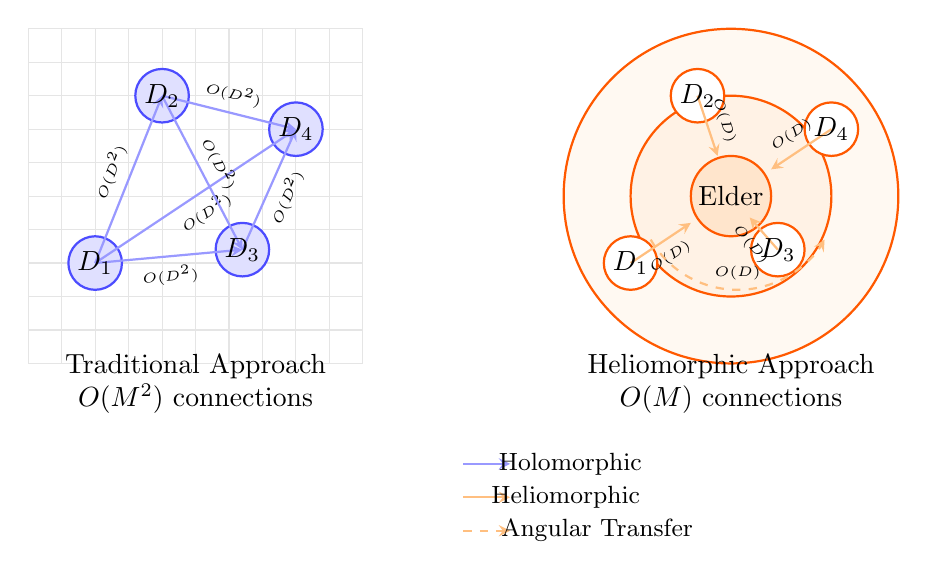
\begin{tikzpicture}[scale=0.85]
  % Define colors
  \colorlet{holocolor}{blue!40}
  \colorlet{heliocolor}{orange!50}
  \colorlet{holoborder}{blue!70}
  \colorlet{helioborder}{orange!70!red}
  
  % Holomorphic diagram (left side)
  \begin{scope}[shift={(-4,0)}]
    % Background grid for traditional approach
    \draw[step=0.5, black!10, thin] (-2.5,-2.5) grid (2.5,2.5);
    
    % Domain circles
    \draw[fill=holocolor!30, draw=holoborder, thick] (-1.5,-1) circle (0.4);
    \draw[fill=holocolor!30, draw=holoborder, thick] (-0.5,1.5) circle (0.4);
    \draw[fill=holocolor!30, draw=holoborder, thick] (0.7,-0.8) circle (0.4);
    \draw[fill=holocolor!30, draw=holoborder, thick] (1.5,1) circle (0.4);
    
    % Cross-domain interactions (all connected)
    \draw[->, thick, >=stealth, draw=holocolor] (-1.5,-1) -- node[sloped, above, font=\tiny] {$O(D^2)$} (-0.5,1.5);
    \draw[->, thick, >=stealth, draw=holocolor] (-1.5,-1) -- node[sloped, below, font=\tiny] {$O(D^2)$} (0.7,-0.8);
    \draw[->, thick, >=stealth, draw=holocolor] (-1.5,-1) -- node[sloped, below, font=\tiny] {$O(D^2)$} (1.5,1);
    \draw[->, thick, >=stealth, draw=holocolor] (-0.5,1.5) -- node[sloped, above, font=\tiny] {$O(D^2)$} (0.7,-0.8);
    \draw[->, thick, >=stealth, draw=holocolor] (-0.5,1.5) -- node[sloped, above, font=\tiny] {$O(D^2)$} (1.5,1);
    \draw[->, thick, >=stealth, draw=holocolor] (0.7,-0.8) -- node[sloped, below, font=\tiny] {$O(D^2)$} (1.5,1);
    
    % Labels
    \node at (-1.5,-1) {$D_1$};
    \node at (-0.5,1.5) {$D_2$};
    \node at (0.7,-0.8) {$D_3$};
    \node at (1.5,1) {$D_4$};
    
    \node[align=center] at (0,-2.8) {Traditional Approach\\ $O(M^2)$ connections};
  \end{scope}
  
  % Heliomorphic diagram (right side)
  \begin{scope}[shift={(4,0)}]
    % Concentric circles for shells
    \draw[fill=heliocolor!10, draw=helioborder, thick] (0,0) circle (2.5);
    \draw[fill=heliocolor!20, draw=helioborder, thick] (0,0) circle (1.5);
    \draw[fill=heliocolor!40, draw=helioborder, thick] (0,0) circle (0.6);
    
    % Domain positions on shells
    \filldraw[fill=white, draw=helioborder, thick] (-1.5,-1) circle (0.4);
    \filldraw[fill=white, draw=helioborder, thick] (-0.5,1.5) circle (0.4);
    \filldraw[fill=white, draw=helioborder, thick] (0.7,-0.8) circle (0.4);
    \filldraw[fill=white, draw=helioborder, thick] (1.5,1) circle (0.4);
    
    % Radial connections only (much fewer)
    \draw[->, thick, >=stealth, draw=heliocolor] (-1.5,-1) -- node[sloped, below, font=\tiny] {$O(D)$} (-0.6,-0.4);
    \draw[->, thick, >=stealth, draw=heliocolor] (-0.5,1.5) -- node[sloped, above, font=\tiny] {$O(D)$} (-0.2,0.6);
    \draw[->, thick, >=stealth, draw=heliocolor] (0.7,-0.8) -- node[sloped, below, font=\tiny] {$O(D)$} (0.28,-0.32);
    \draw[->, thick, >=stealth, draw=heliocolor] (1.5,1) -- node[sloped, above, font=\tiny] {$O(D)$} (0.6,0.4);
    
    % Angular connections on same shell
    \draw[->, thick, >=stealth, draw=heliocolor, dashed] (-1.2,-0.65) arc (-150:-30:1.5) node[pos=0.5, sloped, above, font=\tiny] {$O(D)$};
    
    % Labels
    \node at (-1.5,-1) {$D_1$};
    \node at (-0.5,1.5) {$D_2$};
    \node at (0.7,-0.8) {$D_3$};
    \node at (1.5,1) {$D_4$};
    \node at (0,0) {Elder};
    
    \node[align=center] at (0,-2.8) {Heliomorphic Approach\\ $O(M)$ connections};
  \end{scope}
  
  % Legends
  \begin{scope}[shift={(0,-4)}]
    \draw[->, thick, >=stealth, draw=holocolor] (0,0) -- (0.7,0);
    \node[align=left, font=\small] at (1.6,0) {Holomorphic};
    
    \draw[->, thick, >=stealth, draw=heliocolor] (0,-0.5) -- (0.7,-0.5);
    \node[align=left, font=\small] at (1.53,-0.5) {Heliomorphic};
    
    \draw[->, thick, >=stealth, draw=heliocolor, dashed] (0,-1) -- (0.7,-1);
    \node[align=left, font=\small] at (2,-1) {Angular Transfer};
  \end{scope}
\end{tikzpicture}